\documentclass[12pt]{Article}

% Package to handle graphics inclusion (optional)
\usepackage{graphicx}
% Package for better math formatting (optional)
\usepackage{amsmath}
% For references (optional)
\usepackage{cite}
% Package to customize title position
\usepackage{titling}
\usepackage{subcaption}
\usepackage{listings}
\usepackage{xcolor}
\usepackage{hyperref}

\lstset{
    language=Python,
    basicstyle=\ttfamily\small,
    keywordstyle=\color{blue},
    commentstyle=\color{gray},
    stringstyle=\color{red},
    showstringspaces=false,
    numbers=left,
    numberstyle=\tiny\color{gray},
    breaklines=true,
    frame=single,
    captionpos=b
}


\usepackage{silence}
\usepackage{wrapfig}
\usepackage{float}
\usepackage{adjustbox}
\usepackage[margin=0.8in]{geometry}  % Adjust the margin as needed

\setlength{\parindent}{15pt} 
% Adjust the title position
\setlength{\droptitle}{-6em}% Adjust the value as needed
% Title and Author information
\title{Lab 8 - Deploy over Digital Ocean hosted Kubernetes}
\author{
    Hugo Garrido-Lestache
}
\date{\today \\ CSC 5201 301}

\begin{document}

\maketitle
\section*{Introduction}
In this lab I will be creating a web app micro service and deploying it over a Digital Ocean hosted Kubernetes cluster.
The web app will be a simple chat application that allows you to send messages to a chat room.
It will be using a sql database to store the messages and a redis cache to store the users.

\section{Creating the app}
First I created the app using flask and the code given to me by the professor.
I added functions to add messages to the database, update the username and color of the user, and get the list of messages from the database.   
From this I used AI to create a pretty frontend that allows you to send messages, update your username and color, and see the list of messages. 
After this I ran the app locally to make sure it was working.
Below is a screenshot of the app in action in figure \ref{fig:app}.

\begin{figure}[H]
    \centering
    \fbox{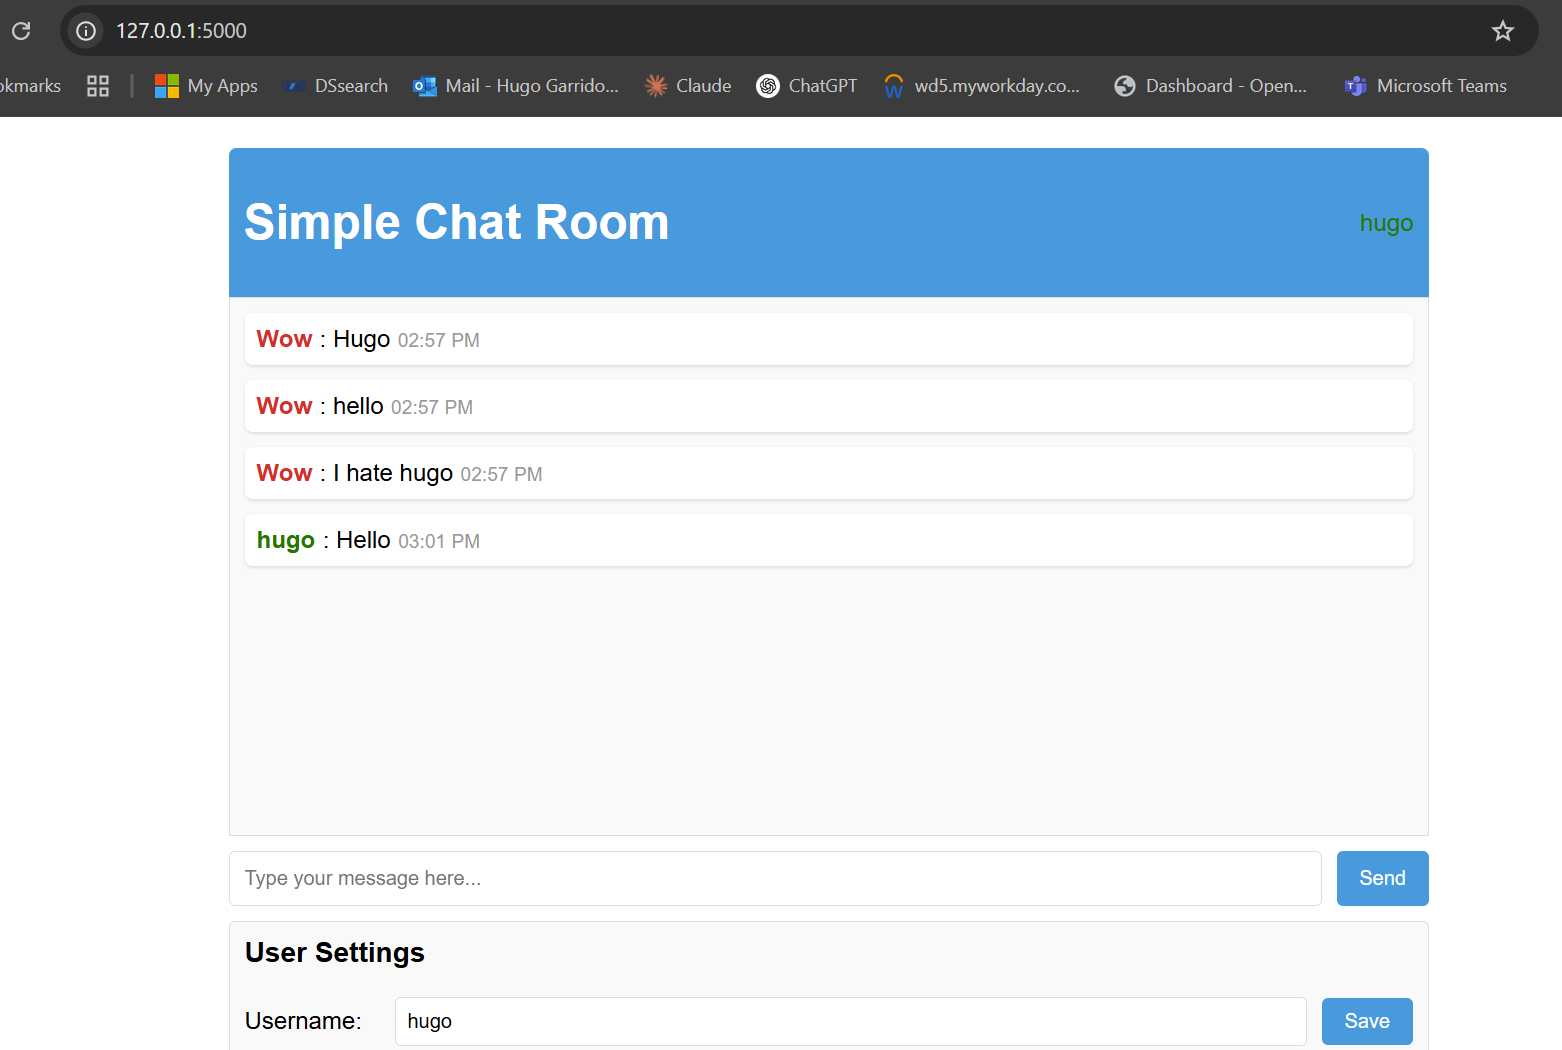
\includegraphics[width=0.8\textwidth]{images/1.png}}
    \caption{Local testing}
    \label{fig:app}
\end{figure}

\section{Pushing to Digital Ocean registry}
After this I created a docker file to containerize the app.
I went to digital ocean and created a container registry.
After setting up the computer to have the correct credentials I was able to push the image to the registry.
After this I ran the app from the digital ocean container registry and it worked as expected.
Below is a screenshot of the app being ran from the digital ocean container registry in figure \ref{fig:app}.

\begin{figure}[H]
    \centering
    \fbox{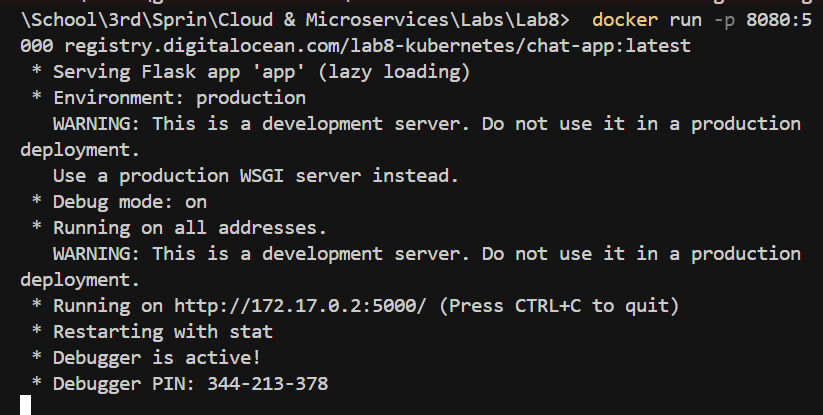
\includegraphics[width=0.8\textwidth]{images/2.png}}
    \caption{Digital Ocean testing}
    \label{fig:app}
\end{figure}

\section{Deploying to Kubernetes}
After this I created a kubernetes cluster on digital ocean.
I gave the cluster permission to access the container registry.
I then created a deployment and a service to deploy the app to the cluster.
Below is a screenshot of the app being ran from the kubernetes cluster in figure \ref{fig:app}.

\begin{figure}[H]
    \centering
    \fbox{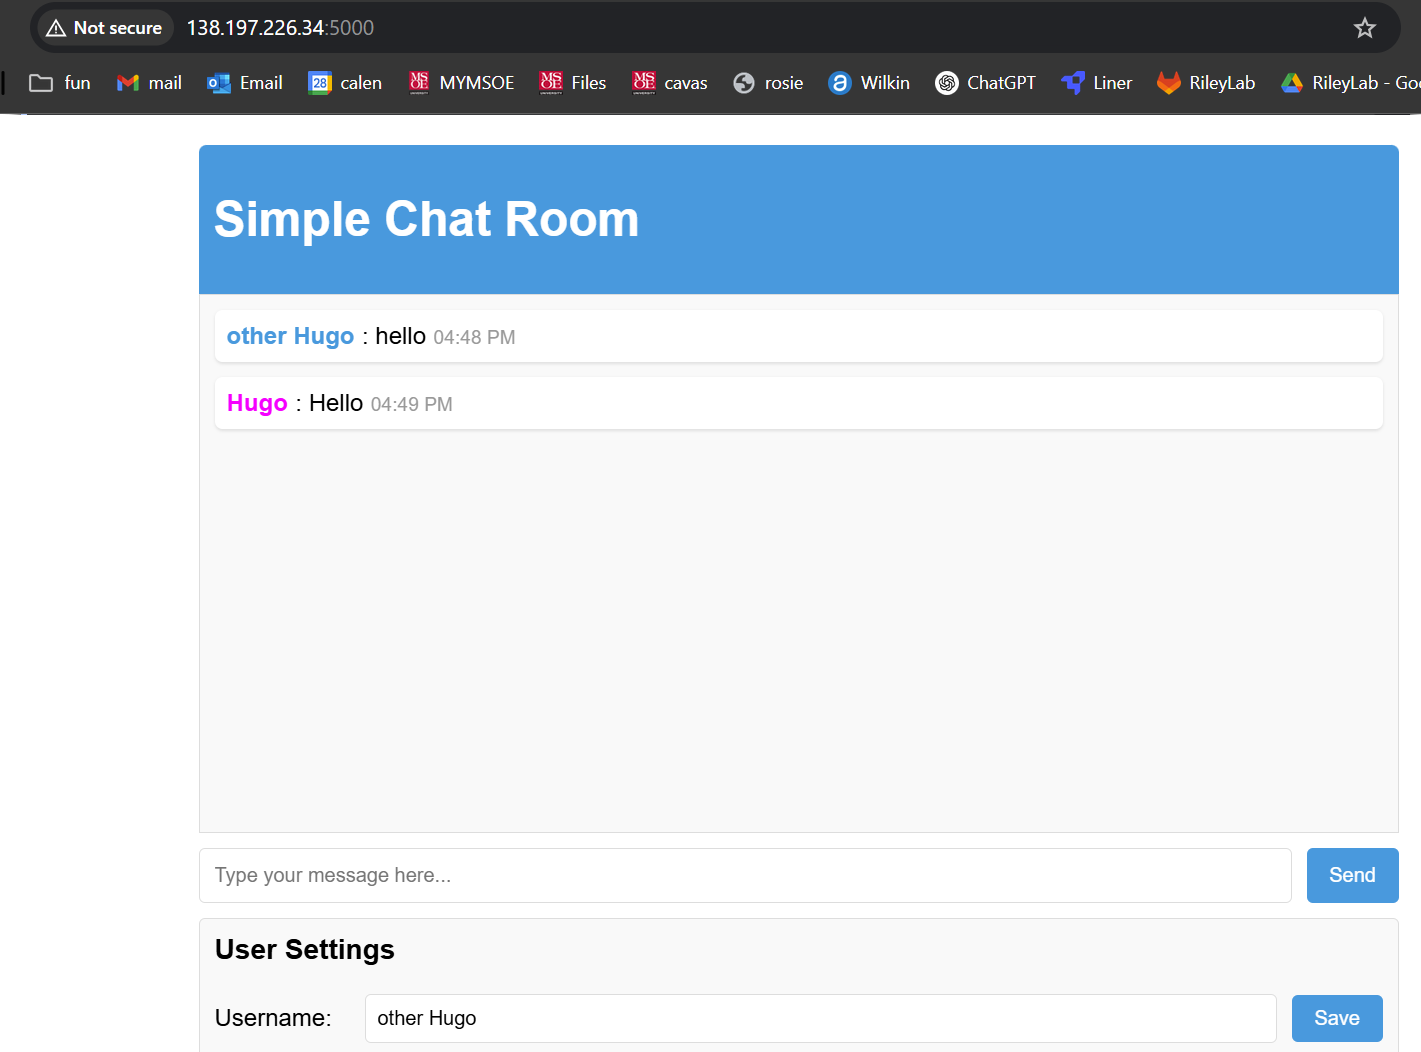
\includegraphics[width=0.8\textwidth]{images/3.png}}
    \caption{Kubernetes testing}
    \label{fig:app}
\end{figure}

\section{Testing the app}
After this I tested the app by sending messages and updating the username and color.
below is a screenshot of me sending a message in the app in figure \ref{fig:app}.

\begin{figure}[H]
    \centering
    \fbox{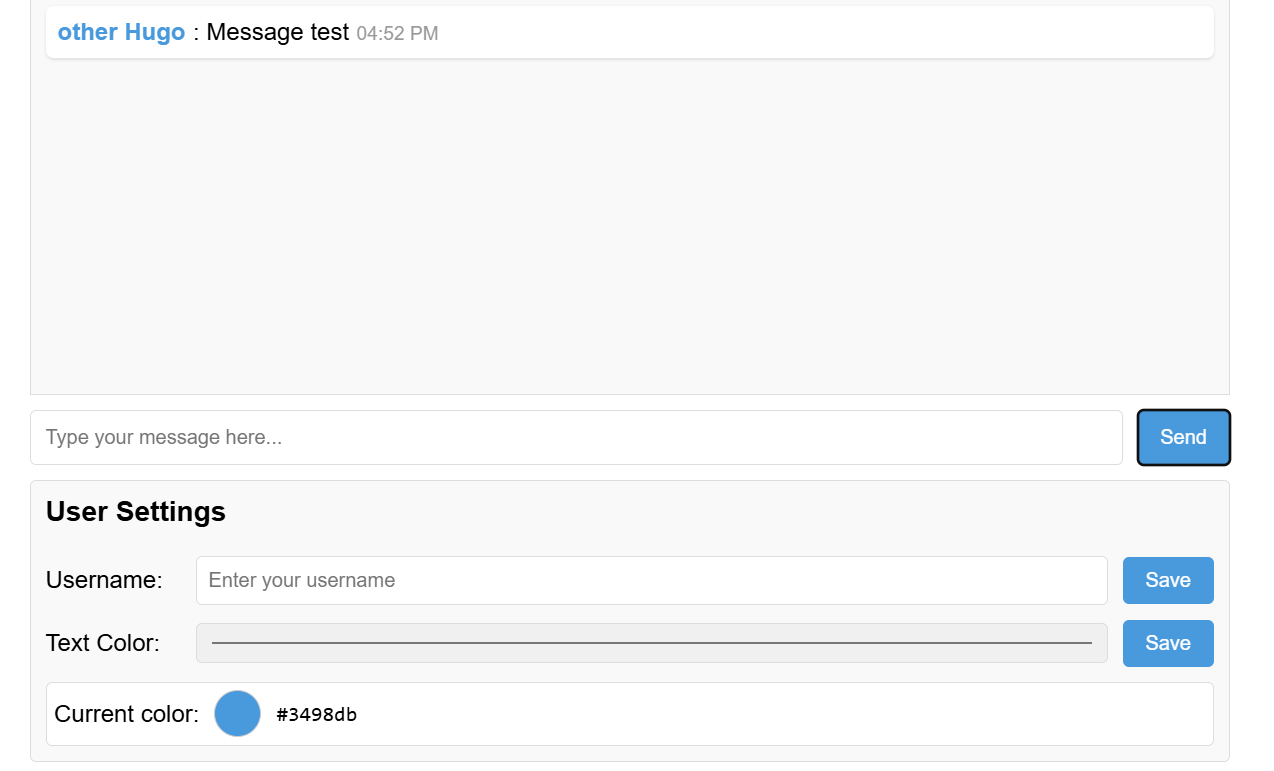
\includegraphics[width=0.8\textwidth]{images/4.png}}
    \caption{Testing the app}
    \label{fig:app}
\end{figure}

I then changed the username to ensure that it was working.
Below is a screenshot of the app with the username changed in figure \ref{fig:app}.

\begin{figure}[H]
    \centering
    \fbox{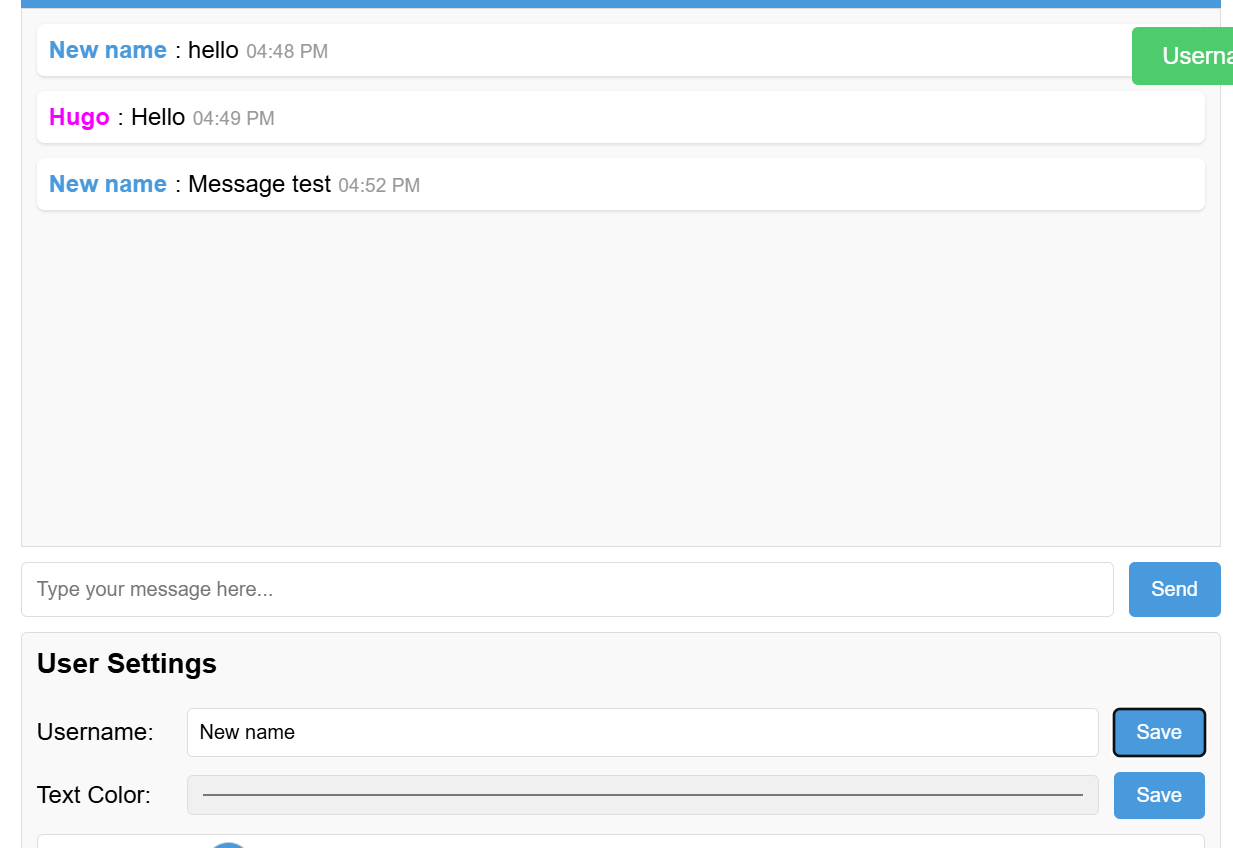
\includegraphics[width=0.8\textwidth]{images/5.png}}
    \caption{Username change}
    \label{fig:app}
\end{figure}

After that I changed the color of the user to ensure that it was working.
Below is a screenshot of the app with the color changed in figure \ref{fig:app}.

\begin{figure}[H]
    \centering
    \fbox{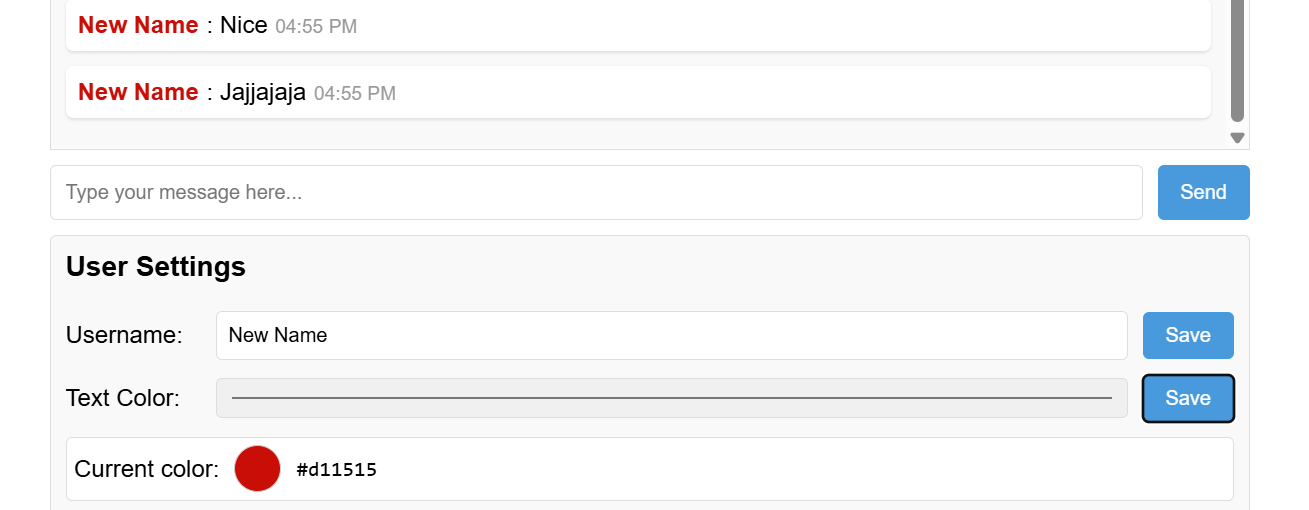
\includegraphics[width=0.8\textwidth]{images/6.png}}
    \caption{Color change}
    \label{fig:app}
\end{figure}

I then send the link to my friends and we all were able to have a conversation together which was fun.

\section*{feedback}
This lab was fun and intresting for learning how to deploy a flask app to a kubernetes cluster.
I think the instructions were good and built on the previous labs to help us understand the concepts better.
I had issues pushing the image and running the kubernetes cluster, I found that storing the my digital ocean key to the enviroment vairables seemed to fix the issue.
Despite this I think the lab was very good.
Going forward I would consider giving labs with less direction allowing us to research and figure out the methods on our own.
This might be challenging for some students but I think being able to figure out the methods on our own would be very helpful.  


\section*{Repo Link}
\href{https://github.com/Hugogales/lab8-kubernetes}{https://github.com/Hugogales/lab8-kubernetes}

\end{document}
